\documentclass[10pt,letterpaper,english]{article}
\usepackage{mathpazo}
\usepackage[hmargin=2cm,vmargin=2cm]{geometry}
\usepackage{graphicx}
\usepackage{marvosym}
\usepackage{subfigure}
\usepackage{amsmath}
\usepackage{multicol}
\usepackage{float}
\usepackage{booktabs}
\usepackage{enumerate}
\usepackage{dingbat}
\usepackage{tikz-timing}[2009/05/15]
\usepackage{amsthm}% http://ctan.org/pkg/amsthm
\renewcommand*\thesection{\arabic{section}.0}
\usepackage{pdfpages}
\usepackage{calc}
\usetikzlibrary{circuits.logic.US,calc, positioning}
\usepackage{tikz-timing}
%\renewcommand{\familydefault}{\sfdefault}
%\usepackage{helvet}
\usepackage{babel}
\usepackage{fancyhdr}
\pagestyle{empty}
\usepackage[compact]{titlesec}
\titlespacing{\section}{0pt}{2ex}{1ex}
\titlespacing{\subsection}{0pt}{2ex}{1ex}
\titlespacing{\subsubsection}{0pt}{0.4ex}{0ex}


  \hyphenpenalty=500000
  \tolerance=1000

% indentsection style, used for sections that aren't already in lists
% that need indentation to the level of all text in the document
\newenvironment{indentsection}[1]{\begin{list}{}%
{\setlength{\leftmargin}{#1}}%
\item[]%
}{\end{list}}

% opposite of above; bump a section back toward the left margin
\newenvironment{unindentsection}[1]{\begin{list}{}%
{\setlength{\leftmargin}{-0.5#1}}%
\item[]%
}{\end{list}}

% format two pieces of text, one left aligned and one right aligned
\newcommand{\headerrow}[2]{\begin{tabular*}{\linewidth}[t]{l@{\extracolsep{\fill}}r}
#1 &
#2 \\
\end{tabular*}}

\thispagestyle{fancy}
\renewcommand{\headrulewidth}{0pt}
\rfoot{Prepared by HSV, DJS, RDN}    
\cfoot{}
\begin{document}

\textsc{op-amps}\\
% refer to here zebu.uoregon.edu/~rayfrey/431/notes9.pdf
Virtual short: V+ = V-\\
High imput impedance ($\infty$)\\
\textsc{basic configurations}
\begin{multicols}{2}
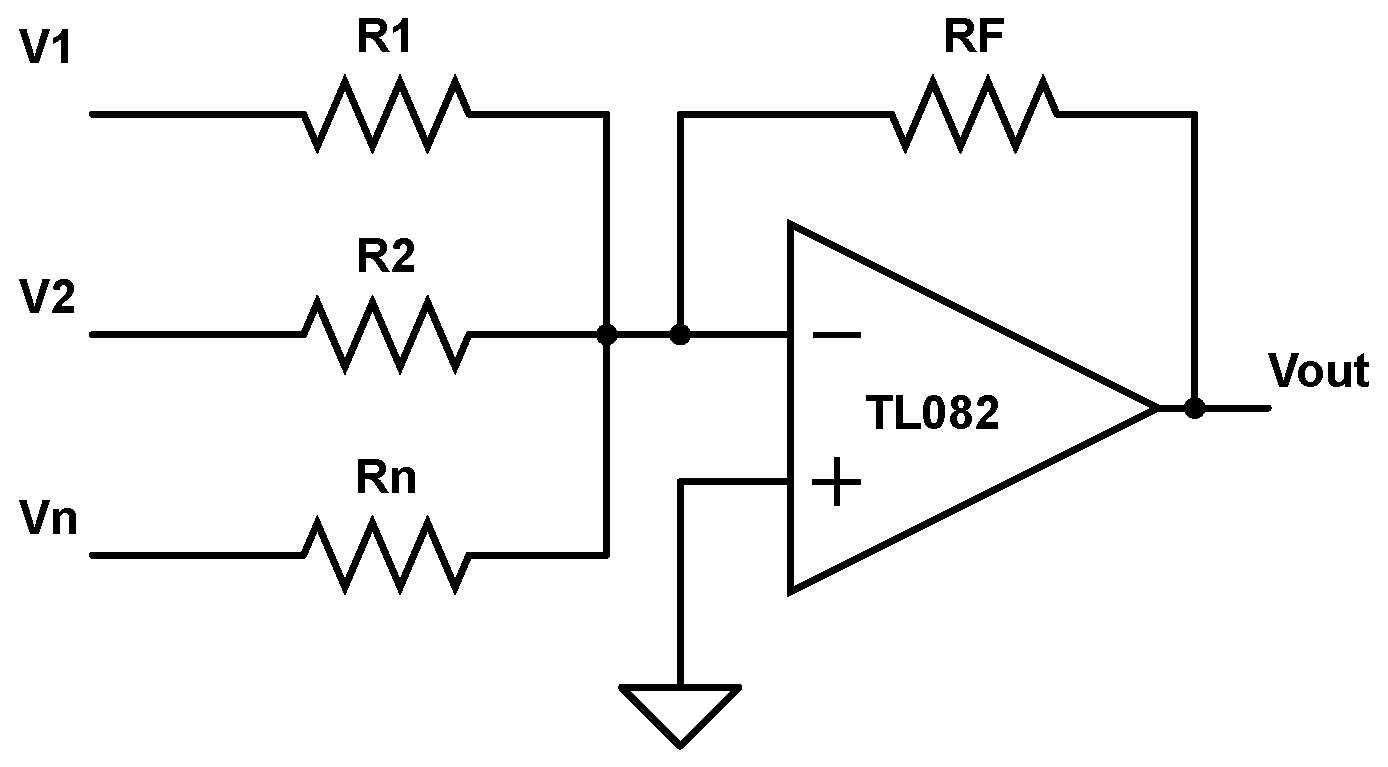
\includegraphics[scale=0.2]{opamp-1.eps}
\begin{align*}
V_{out} = -\left(\frac{R_F}{R_1}\cdot V_1 + \frac{R_F}{R_2}\cdot V_2 \cdots + \frac{R_F}{R_n}\cdot V_n\right)\\
V_n\rightarrow R_n\rightarrow Op-, OP- \rightarrow R_F \rightarrow V_{out}
\end{align*}
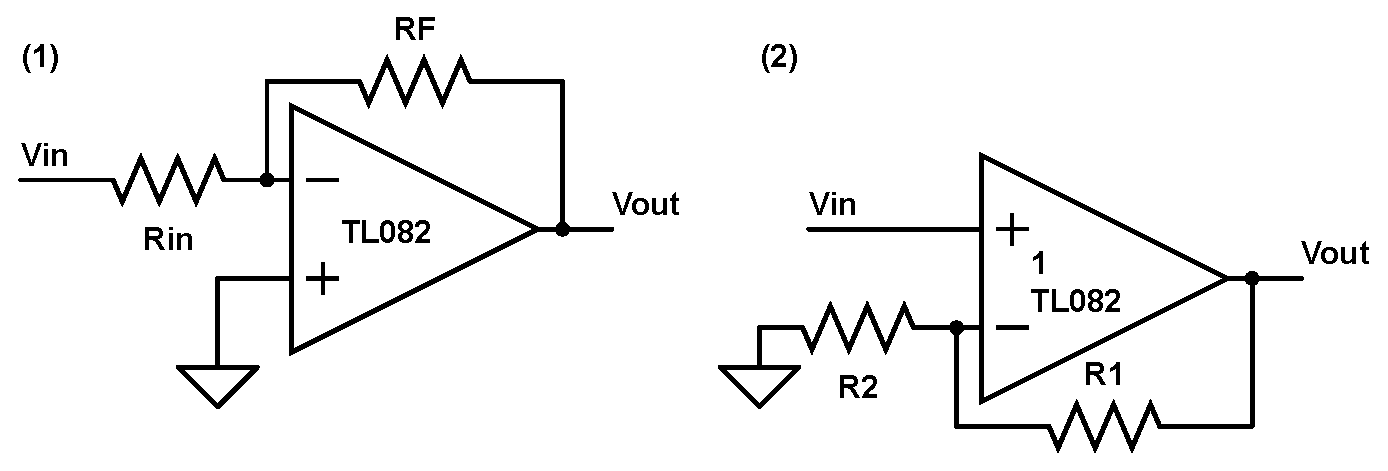
\includegraphics[scale=0.4]{opamp-2.eps}
\begin{align*}
V_{out} = -\frac{R_F}{R_{in}}\cdot V_{in} \tag*{(1) Inverting}\\
V_{in}\rightarrow R_{in} \rightarrow Op-, Op- \rightarrow R_F \rightarrow V_{out}\\
V_{out} = \left(1 + \frac{R_1}{R_2}\right)\cdot V_{in} \tag*{(2) Non-inverting}\\
V_{in}\rightarrow Op+, GND \rightarrow R_2 \rightarrow Op-, Op- \rightarrow R_1 \rightarrow V_{out}\\
\end{align*}
\end{multicols}


\begin{multicols}{2}
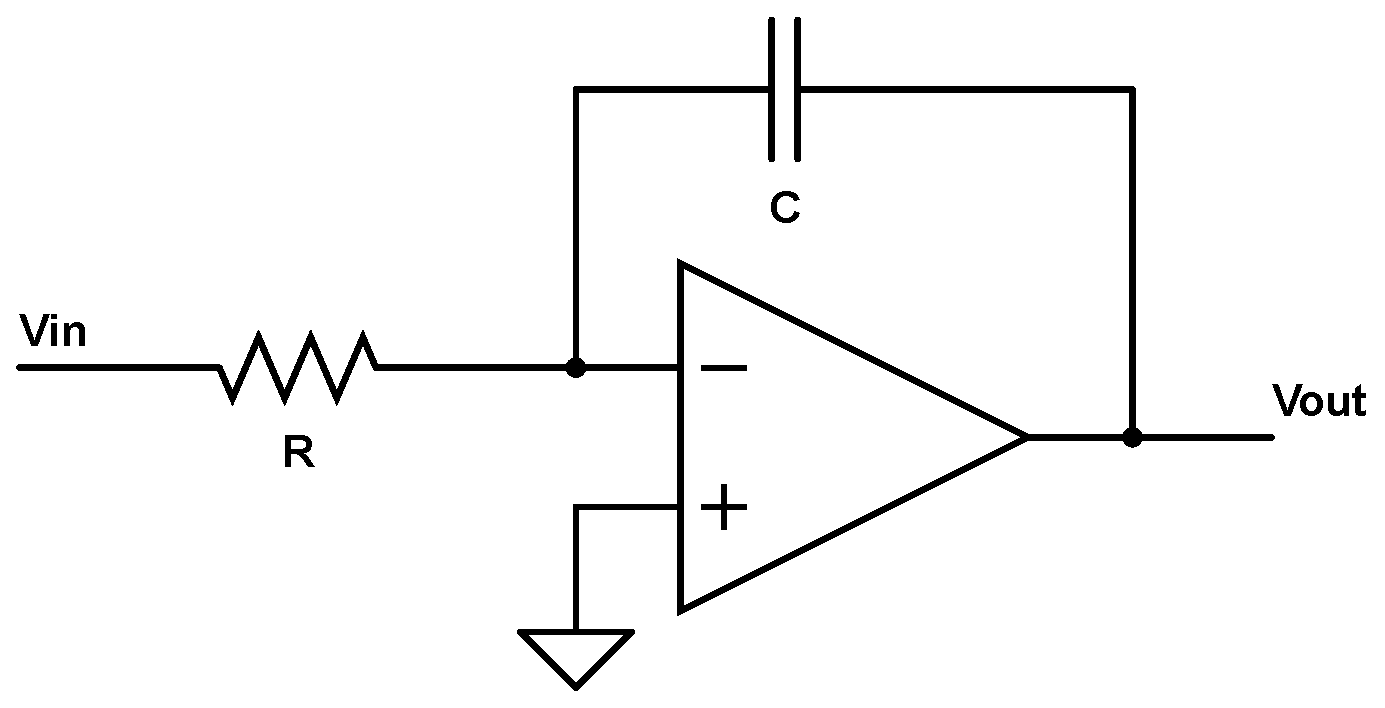
\includegraphics[scale=0.2]{opamp-integrator.eps}
\begin{align*}
V_{out} = -\int_0^t \frac{V_{in}}{RC} \,dt; \frac{V_{out}}{V_{in}} = \frac{-1}{j \omega RC} \tag*{Miller Integrator / Low-pass}\\
V_{in}\rightarrow Op- \rightarrow C \rightarrow V_{out}, O+ \rightarrow GND
\end{align*}
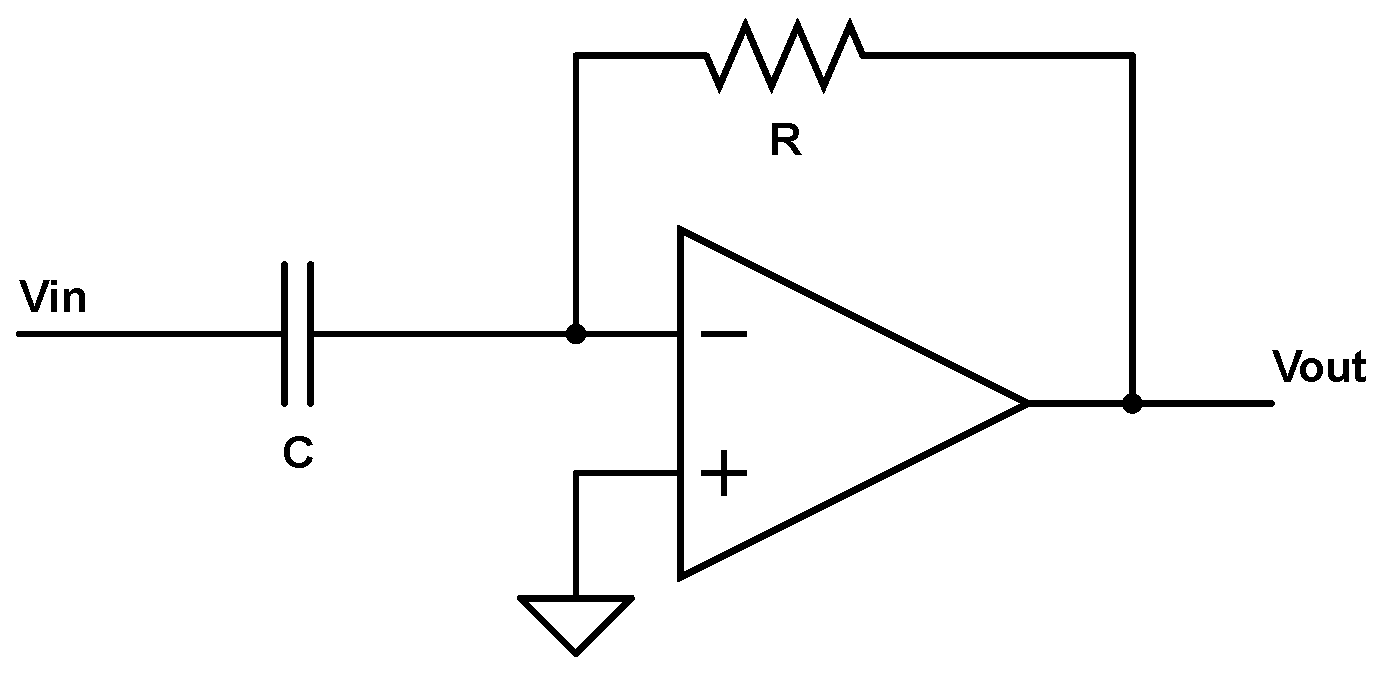
\includegraphics[scale=0.2]{opamp-differentiator.eps}
\begin{align*}
V_{out} = -RC \frac{\,dV_{in}}{\,dt} \tag*{Differentiator / High-pass}\\
\end{align*}
\end{multicols}


\textsc{mosfets}\\

\begin{multicols}{2}
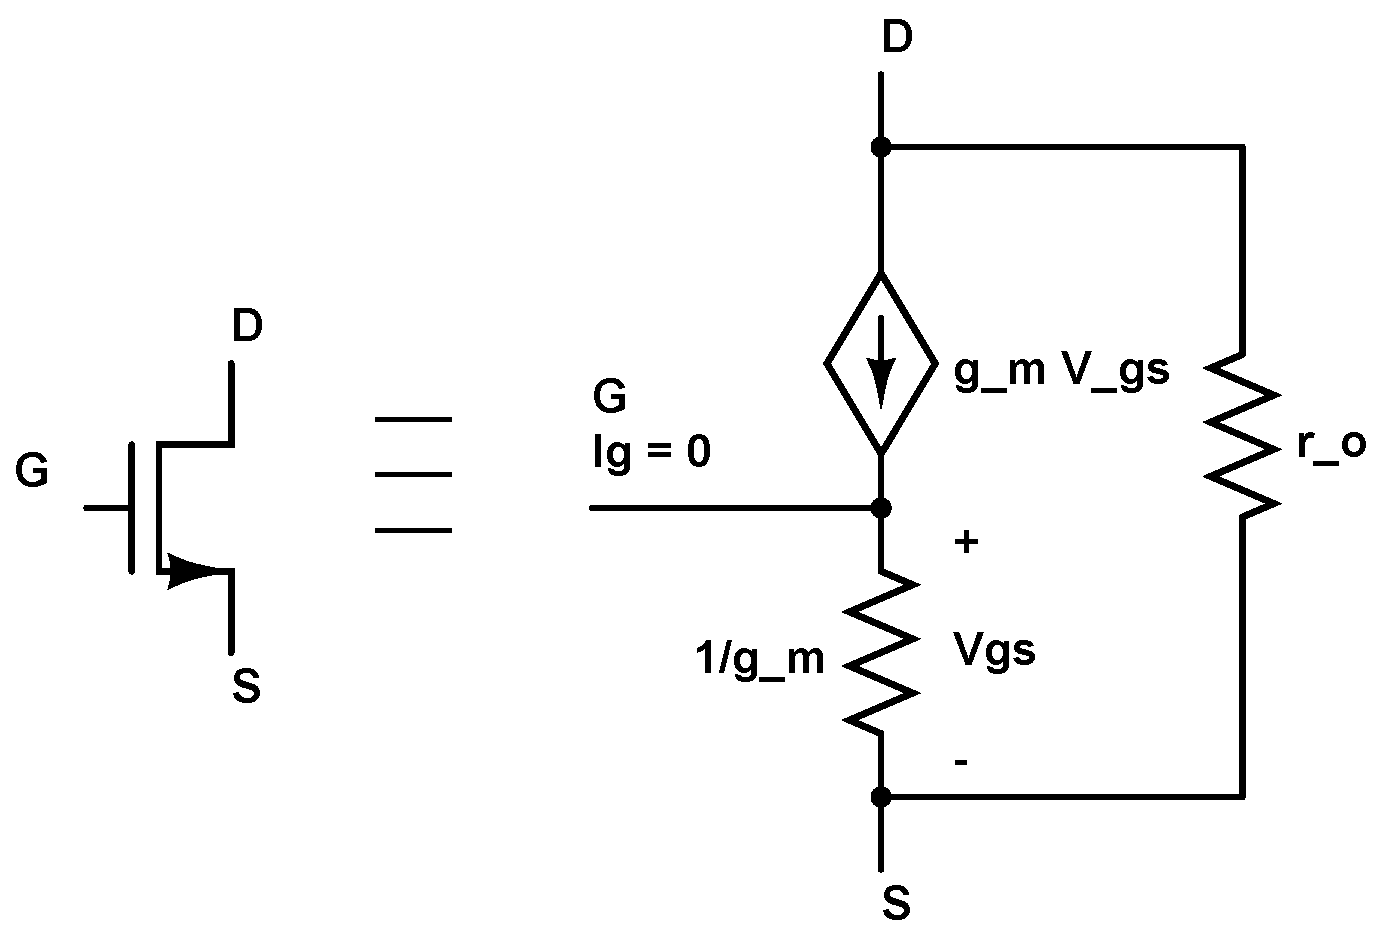
\includegraphics[scale=0.24]{mosfet-t-model.eps}
\begin{align*}
\tag*{Mosfet T-model}\\
\end{align*}
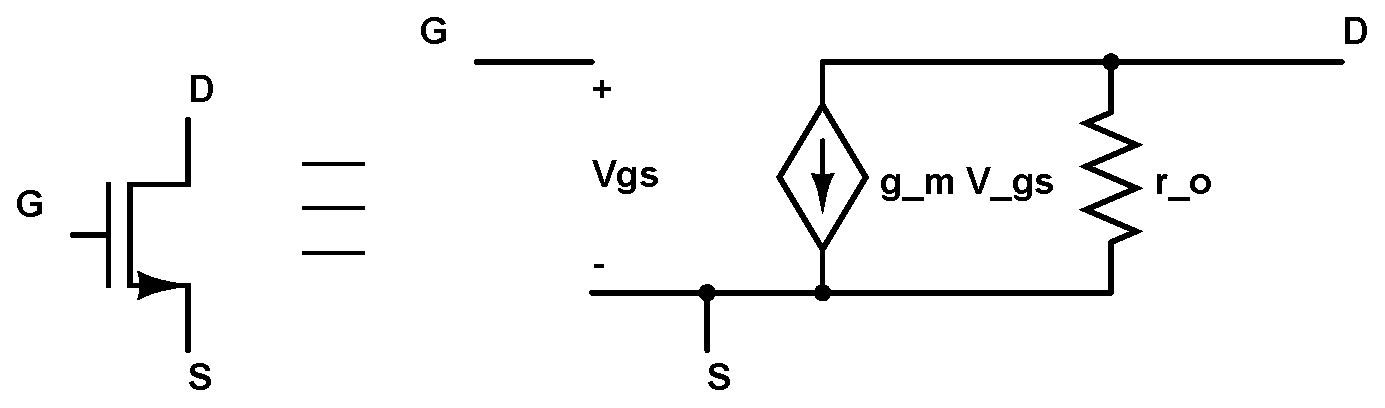
\includegraphics[scale=0.4]{mosfet-hybrid-pi.eps}
\vspace{2mm}
\begin{align*}
A_v = \frac{-g_mr_{out}}{(1 + g_mR_S)} \tag*{Mosfet hybrid pi model}\\
\end{align*}
\end{multicols}


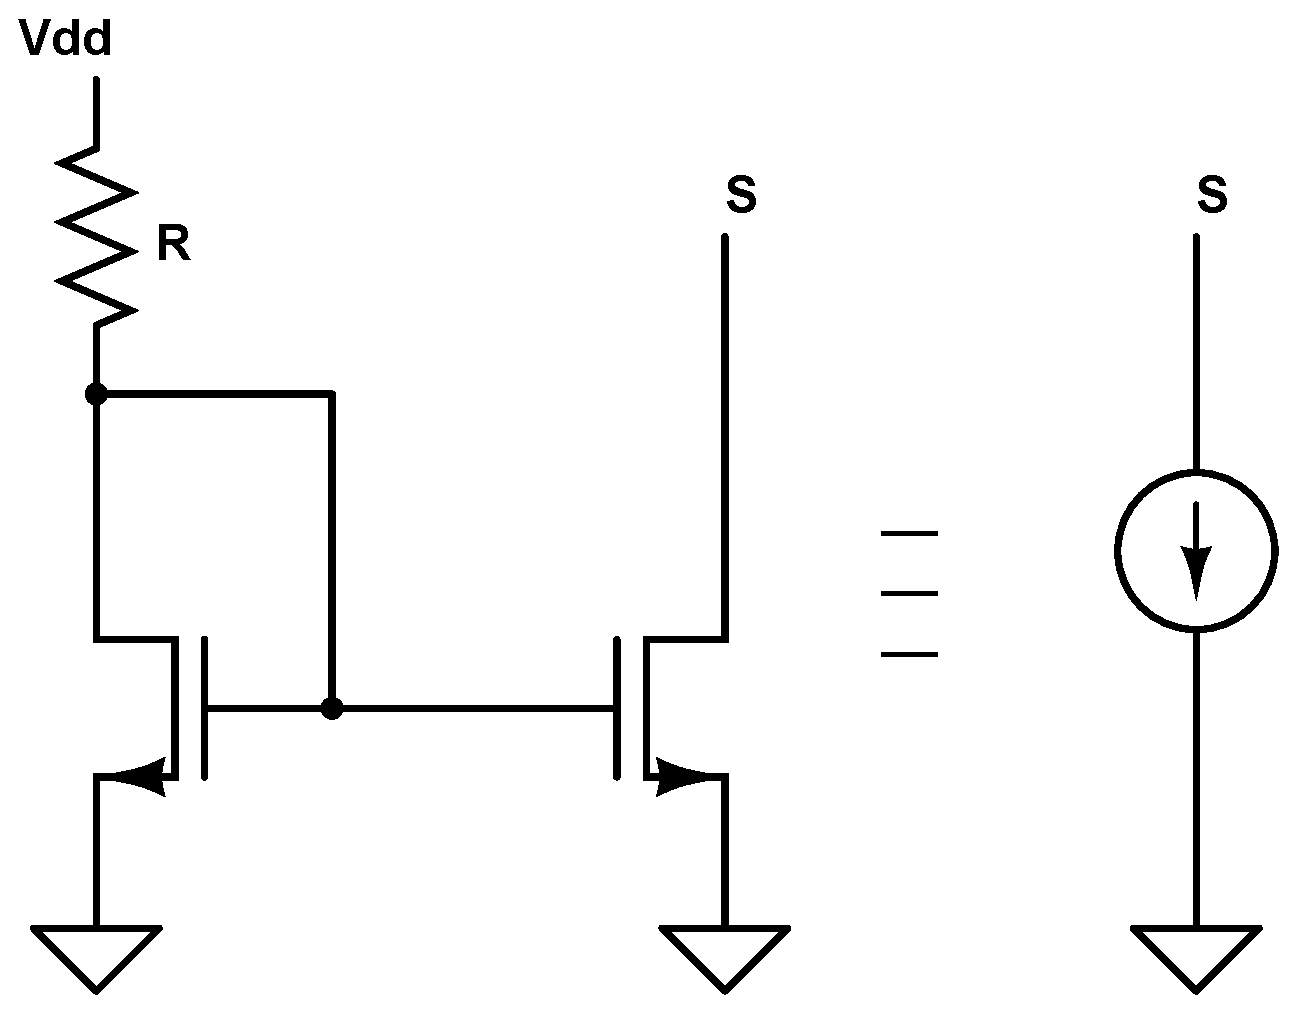
\includegraphics[scale=0.2]{mosfet-current-mirror.eps}
\begin{align*}
I_{current\ source}&= \frac{W_2/L_2}{W_1/L_1}\cdot I_{REF} \tag*{MOSFET current mirror circuit}
\end{align*}


\textsc{diodes}\\
\begin{multicols}{2}
\begin{enumerate}
\item{Clipper: clips one part of signal, voltage across single diode. $V_o+ \leq V_B, V_o- = V_i$ or $V_o+ \leq V_B, V_o- \geq V_i-$}
 \item{Clamper: shifts signal's DC component.}
\end{enumerate}
\begin{align*}
\textsc{Shockley Diode Eqn:}\\
I= I_S\left(e^{\frac{V_D}{\left(nV_t\right)}} - 1\right)\nonumber\\
\textsc{Zener Diode Voltage Drop:}\\
V_{Z} = V_{Z0} + i_Zr_Z\nonumber\\
\end{align*}
\end{multicols}

\textsc{MOSFETs}\\
\begin{multicols}{2}
\begin{align*}
g_m& = \sqrt{2\mu_n \cdot C_{ox}\frac{W}{L} \cdot I_d} = \sqrt{2I_D\cdot K}\\
K&= \mu_n \cdot C_{ox}\frac{W}{L} \\
\lambda&= \frac{1}{|V_A|}, r_o= \frac{|V_A|}{I_D}\\
I_D&= K\left((V_{GS} - V_t)V_{DS} -\frac{V_{DS}}{2}\right),triode\\
I_D&= \frac{K}{2}\left((V_{GS} - V_t)^{2}\right) sat\\
g_m&=\left.\frac{\partial i_D}{\partial v_{GS}} \right|_{V_{GSQ}} = K\left(V_{GSQ} - V_t\right)\nonumber\\
\end{align*}
Modes of operation:
\begin{enumerate}
\item{Cutoff mode:$V_{GS} < V_t$. Transistor OFF.}
\item{Triode mode: $V_{GS} > V_t, V_{DS} < (V_{GS} - V_t)$, linear resistor}
\item{Saturation mode:$V_{DS} \geq (V_{GS} - V_t), V_{GS} - V_t > 0$, amplifier}
\end{enumerate}
\emph{Notes}\\
NMOS common emitter amplifier produces signal $180^\circ$ out of phase.\\
High input impedance ($R\rightarrow \infty$)
\end{multicols}

\textsc{BJTs}\\
\begin{multicols}{2}
\begin{align*}
I_C&=I_S\cdot e^{\frac{V_{BE}}{V_T}}\nonumber\\
I_C&=\beta \cdot I_B, I_C = \alpha I_E\nonumber\\
\alpha&=\frac{\beta}{\beta + 1}\nonumber\\
g_m& = \frac{I_c}{V_t}\nonumber\\
I_E&= I_C + I_B\nonumber\\
r_\pi&= \frac{V_T}{I_B}, r_0 = \frac{|V_A|}{I_C}\nonumber\\
\end{align*}
\end{multicols}
\end{document}
